\documentclass[11pt]{article}

\usepackage{graphicx}
\usepackage{url}
\usepackage[listings]{tcolorbox}
\usepackage{amssymb}
\usepackage{pifont}

\newcommand{\critics}{{\small{\sc{Critics}}}}
\newcommand{\phabricator}{{\small{\sc{Phabricator}}}}
\newcommand{\gerrit}{{\small{\sc{Gerrit}}}}
\newcommand{\codeflow}{{\small{\sc{CodeFlow}}}}
\newcommand{\collaborator}{{\small{\sc{Collaborator}}}}
\newcommand{\clusterchanges}{{\small{\sc{ClusterChanges}}}}
\newcommand{\delCode}{\textcolor{black}}
\newcommand{\addCode}{\textcolor{black}}
\newcommand{\ttt}[1]{\tt\small{#1}}


% -----------------------------------------------------------------
% color
% -----------------------------------------------------------------
\definecolor{javared}{rgb}{0.6,0,0} % for strings
\definecolor{javagreen}{rgb}{0.25,0.5,0.35} % comments
\definecolor{javapurple}{rgb}{0.5,0,0.35} % keywords
\definecolor{javadocblue}{rgb}{0.25,0.35,0.75} % javadoc

% ===============================================
% MyJavaSmallStyle
% ===============================================
\lstdefinestyle{MyJavaSmallStyle} {
  language=Java,
  frame=none,
  xleftmargin=15pt, 
  stepnumber=1, 
  numbers=left, 
  numbersep=5pt,
  numberstyle=\tiny\color[gray]{0.777}, 
  belowcaptionskip=\bigskipamount,
  captionpos=b, 
  escapeinside={*'}{'*},
  tabsize=5,
  emphstyle={\bf},
  basicstyle=\scriptsize\ttfamily,
  keywordstyle=\color{javapurple}\bfseries,
  stringstyle=\color{javared},
  commentstyle=\color{javagreen},
  morecomment=[s][\color{javadocblue}]{/**}{*/},
  showspaces=false,
  columns=flexible,
  showstringspaces=false,
  morecomment=[l]{//},
  tabsize=2,
  morekeywords={, Package,Invariant,Class,Method,Field,Where,in,Assert,ToLc,Split,Msg,Immutable,<<<,eq,neq,not,has,Assert,AssertExists,Attribute,Uc,Lc,},
  breaklines=true
}

\begin{document}

\section{Modern Code Review}

Peer code review is a quality assurance mechanism that requires software developers to manually inspect each other's source code to find programming mistakes overlooked in the initial development phase. In 1976, Fagan formalized code review as a highly structured inspection process with multiple stages (e.g., {\em overview}, {\em preparation}, {\em inspection}, {\em rework}, {\em follow-up}) and multiple participants (e.g., {\em moderator}, {\em designer}, {\em implementor}, and {\em tester})~\cite{fagan2001design}. This inspection process is performed at the end of each software development phase (e.g., design, implementing, testing), in which software developers attend a series of group meetings and review design documentations and source code line by line. Such careful and thorough inspection process has been proven effective in terms of finding bugs, but the cumbersome and time-consuming nature of this process hinders its universal adoption in practice. 

\begin{figure}[ht]
 \centering
 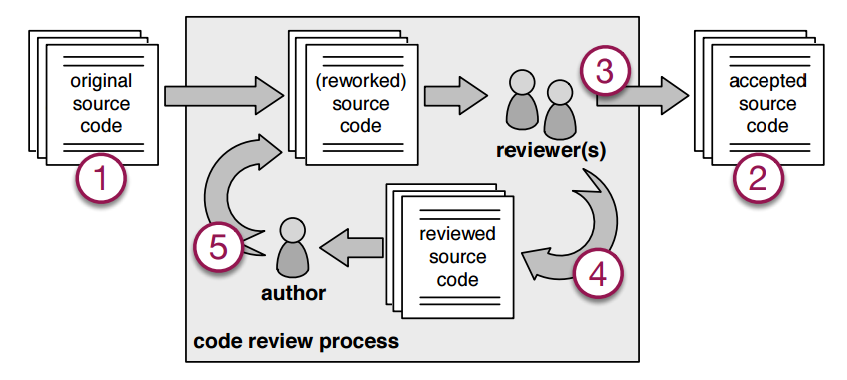
\includegraphics[width=0.8\textwidth]{review-process.png}
 \caption{The modern code review process (based on~\cite{beller2014modern})}
 \label{fig:review-process}
\end{figure}

Nowadays many organizations adopt lightweight code review processes with less overhead than formal code inspections. In contrast to formal code review, modern code review occurs more regularly (often on a daily basis) and does not require a dedicated code review team with particular members. In particular, there is a clear trend towards utilizing code review tools to support code review tasks, instead of organizing and attending group meetings. Figure~\ref{fig:review-process} shows the overall process of a code review task. The {\em author} first submits the {\em original source code} for review. The {\em reviewers} then decide whether the submitted code meets the project's quality acceptance criteria. If not, reviewers can add review comments to the source code and send the {\em reviewed source code} back to the author. The author then revises the source code to address reviewers' comments and then send it back for further review. This process continues till all reviewers accept the revised source code. Modern code review is widely practiced both in open-source and industrial contexts and is recognized as a valuable tool to remove common vulnerabilities, performance bugs, and style issues. 

Recent studies have investigated the common practices and challenges in modern code review. Rigby et al.~conduct a case study in an open-source software project, Apache HTTP server, using archived code review records in email discussions and version control repositories~\cite{rigby2008open}. They find that, in contrast to traditional software inspection (Fagan style), modern code review in open-source projects often involves frequent review tasks of small yet complete program contributions, conducted asynchronously by a small group of self-selected experts. Rigby and Bird conduct a similar investigation on a more diverse set of software projects, including two two Google-led projects, Android and Chromium OS, three Microsoft projects, Bing, Office, and MS SQL, and internal projects at Advanced Micro Devices (AMD)~\cite{rigby2013convergent}. They find several convergent code review practices that may indicate general principles of modern code review. For example, modern code review often involves two reviewers and is performed regularly and quickly. They also observe the benefits of sharing knowledge across the development team via peer code review. In order to understand the expectations, outcomes, and challenges of modern code review, Bacchelli and Bird observe, interview, and survey software developers at Microsoft and manually classify hundreds of review comments across several Microsoft teams~\cite{bacchelli2013expectations}. They find that, although the top motivation of code review is finding defects, the actual outcomes are less about finding defects than expected: only a small portion of review comments are related to software defects, which mainly cover small, low-level logical issues. A key challenge reported by reviewers is the lack of tool support for code change comprehension during peer code review. Tao et al.~also study the challenges that developers face when they comprehend code changes and find that modern code review tools must support the capability to divide a large chunk of code changes into small, cohesive groups and to filter non-essential changes~\cite{tao2012software}. 

\section{Code Review Techniques}

Code review is effective only when reviewers are able to understand the changes being made. When the information required to inspect code changes is distributed across multiple files, developers find it difficult to inspect code changes~\cite{dunsmore2000object}. For example, when an API gets modified in the latest release, all call sites using this API must be updated correctly. Such edits tend to be systematic\textemdash involving similar but not identical edits to multiple locations.

Unfortunately, popular code review tools\textemdash Facebook's {\phabricator},\footnote{\url{http://phabricator.org}} Google's {\gerrit},\footnote{\url{http://code.google.com/p/gerrit/}} and Microsoft's {\codeflow},\footnote{\url{http://visualstudioextensions.vlasovstudio.com/2012/01/06/codeflow-code-review-tool-for-visual-studio/}}\textemdash all compute program differences per file. This obliges reviewers to read changed lines file by file, even when those cross-file changes are done systematically to address the same issue. Therefore, reviewers are left to manually inspect individual edits to answer questions such as ``what other code locations are changed similar to this change?'' and ``are there any other locations that are similar to this code but are not updated?''

\begin{figure}[ht]
 \centering
 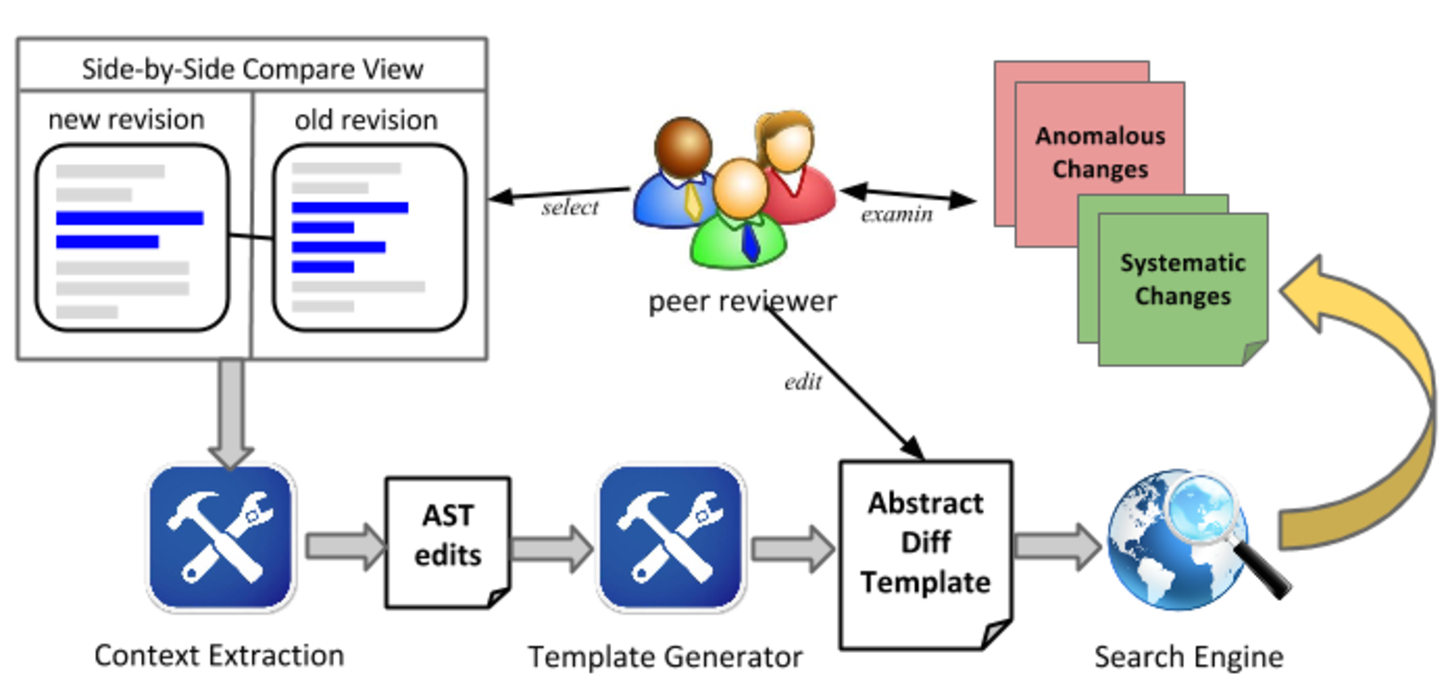
\includegraphics[width=0.8\textwidth]{critics-workflow.pdf}
 \caption{The workflow of {\critics}}
 \label{fig:critics-workflow}
\end{figure}

To address this issue, Zhang et al.~present {\critics}, a novel approach that allows reviewers to interactively inspect such systematic changes during peer code review~\cite{zhang2015interactive}. Figure~\ref{fig:critics-workflow} describes the interactive workflow of {\critics}. Given a specified change that a reviewer would like to inspect, {\critics} creates a change template from the selected change, which serves as the pattern for searching similar changes. {\critics} includes {\em change context} in the template---unchanged, surrounding program statements that are relevant to the selected change. {\critics} models the template as Abstract Syntax Tree (AST) edits and allows reviewers to iteratively customize the template by parameterizing its content and by excluding certain statements. {\critics} then matches the customized template against the rest of the codebase to summarize similar changes and locate potential inconsistent or missing changes. Reviewers can incrementally refine the template and progressively search for similar changes until they are satisfied with the inspection results. This interactive feature allows reviewers with little knowledge of a codebase to flexibly explore the program changes with a desired pattern.

%% =============================================
% !TEX root = ./critics.tex
% =============================================
\begin{figure*}[!t]
%\begin{minipage}[t]{0.5\linewidth}
\begin{lstlisting}[style=MyJavaSmallStyle]
int keyDownEvent (int wParam, int lParam) {
*'\delCode{-}'* *'\delCode{ExpandItem item = items [focusIndex];}'*
  switch (wParam) {
    case OS.VK_RETURN:
      Event event = new Event ();
*'\delCode{-}'*     *'\delCode{event.item = item;}'*
*'\delCode{-}'*     *'\delCode{sendEvent(true, event);}'*
*'\addCode{+}'*     *'\addCode{event.item = focusItem;}'*
*'\addCode{+}'*     *'\addCode{sendEvent(focusItem.expanded ?~COLLAPSE:EXPAND, event);}'*
*'\addCode{+}'*     *'\addCode{refreshItem(focusItem);}'*
    ...
\end{lstlisting}
\vspace{-0.4cm}
\begin{center}\begin{scriptsize}(a) A changed region selected by {\sf Barry}\end{scriptsize}\end{center}
\vspace{-0.4cm}
%\end{minipage}
%
%\begin{minipage}[t]{0.5\linewidth}
\begin{lstlisting}[style=MyJavaSmallStyle]
int keyPressedEvent (int wParam, int lParam) {
  ExpandItem item = items [focusIndex];
  switch (wParam) {
    case OS.VK_RETURN:
      Event event = new Event ();
      event.item = item;
      sendEvent(true, event);
    ...
\end{lstlisting}
\vspace{-0.7cm}
\begin{center}\begin{scriptsize}(b) Code location with exactly the same context but missing the update\end{scriptsize}\end{center}
\vspace{-0.4cm}
%\end{minipage}
%\begin{minipage}[t]{0.5\linewidth}
%
\begin{lstlisting}[style=MyJavaSmallStyle]
int keyReleaseEvent (int wParam, int lParam) {
*'\delCode{-}'* *'\delCode{ExpandItem item = items [focusIndex];}'*
  switch (wParam) {
    case OS.GDK_SPACE:
      Event ev = new Event ();
*'\delCode{-}'*     *'\delCode{ev.item = item;}'*
*'\delCode{-}'*     *'\delCode{sendEvent(true, ev);}'*
*'\addCode{+}'*     *'\addCode{ev.item = focusItem;}'*
*'\addCode{+}'*     *'\addCode{sendEvent(focusItem.expanded ?~COLLAPSE:EXPAND, ev);}'*
*'\addCode{+}'*     *'\addCode{refreshItem(focusItem);}'*
   ...
\end{lstlisting}
\vspace{-0.7cm}
\begin{center}\begin{scriptsize}(c) A similar but not identical change using a different variable name, \texttt{ev}, instead of {\tt event}\end{scriptsize}\end{center}
\vspace{-0.4cm}
%\end{minipage}
%
%\begin{minipage}[t]{0.5\linewidth}
\begin{lstlisting}[style=MyJavaSmallStyle]
int buttonUpEvent (int wParam, int lParam) {
*'\delCode{-}'* *'\delCode{ExpandItem item = items [focusIndex];}'*
  if (lParam == HOVER) {
    Event bEvent = new Event ();
*'\delCode{-}'*   *'\delCode{bEvent.item = item;}'*
*'\delCode{-}'*   *'\delCode{sendEvent(true, bEvent);}'*
*'\addCode{+}'*   *'\addCode{bEvent.item = focusItem;}'*
*'\addCode{+}'*   *'\addCode{sendEvent(focusItem.expanded ?~EXPAND:COLLAPSE, bEvent);}'*
*'\addCode{+}'*   *'\addCode{refreshItem(focusItem);}'*
    ...
\end{lstlisting}
\vspace{-0.7cm}
\begin{center}\begin{scriptsize}(d) Inconsistent change by mistakenly swapping two expressions, {\tt EXPAND} and {\tt COLLAPSE}\end{scriptsize}\end{center}
\vspace{-0.4cm}
%\end{minipage}
\caption{Real-world examples of similar and consistent changes, inconsistent changes, and missing updates, adapted from the revision 13516 in the Eclipse Standard Widget Toolkit (SWT) project. Code deletions are marked with `-' and additions are marked with `+'.}
\label{fig:critics-example}
\end{figure*}


%Now we illustrate {\critics}'s approach in the user's perspective. Suppose Alice updates the program to use the new {\tt sendEvent} API, as shwown in Figure~\ref{fig:critics-example}. Barry needs to review Alice's changes to ensure all locations using {\tt sendEvent} are updated correctly and to check if there is any location that Alice forgot to change. The program changes authored by Alice is over 450 lines, distributed across 42 different locations. 
  
%In order to find incorrect edits, Barry needs to inspect line level differences file by file. In particular, to identify missing updates, he must also inspect unchanged code as well, since the original program differencing output does not show what did {\em not} change. The following shows how Barry may iteratively use {\critics} to inspect similar changes and to detect potential missing or inconsistent updates.    

%\noindent {\bf Iteration 1.} Suppose Barry first inspects changes in the {\tt keyDownEvent} method in Figure~\ref{fig:critics-example}(a). He wonders whether there are other methods that are changed similarly to {\tt keyDownEvent}. So he selects the changed code in the diff patch. Given the selected change, {\critics} identifies the {\em change context}\textemdash unchanged, surrounding code relevant to these edits in terms of control and data dependences, {which further serves} as an anchor to locate missing updates during the searching process. So the default template generated by {\critics} consists of both the initial edit selection and the change context. Using the template, {\critics} locates code that matches the {change context} but is missing the update, shown in Figure~\ref{fig:critics-example}(b).

%\noindent \textbf{Iteration 2.} After examining the search result in the first iteration, Barry wants to explore further since he suspects other locations may use different identifier names. To match similar but not identical changes, {\critics} allows Barry to generalize the change template by parameterizing type, variable, and method names. So Barry generalizes the variable name {\tt event} and searches again. This time, the location in Figure~\ref{fig:critics-example}(c) is summarized although it uses a different variable name, {\tt ev}.

%\noindent \textbf{Iteration 3.} {\critics} includes the change context such as the {\tt switch} and {\tt case} statements from lines 3 to 5 in Figure~\ref{fig:critics-example}(a) in the current template. Barry wonders if there are similar changes in different control-flow contexts such as a {\tt for} loop or an {\tt if-else} branch. He excludes the switch statement. Using the new refined template, {\critics} locates {\tt buttonUpEvent} in Figure~\ref{fig:critics-example}(d). This location uses an {\tt if} statement instead of a {\tt switch} statement. However, {\critics} flags this location as a potential inconsistent change, since Alice mistakenly swapped the two expressions, {\tt EXPAND} and {\tt COLLAPSE}. Such mistake is usually hard for the reviewer to detect during code inspection. 

\begin{figure}[ht]
 \centering
 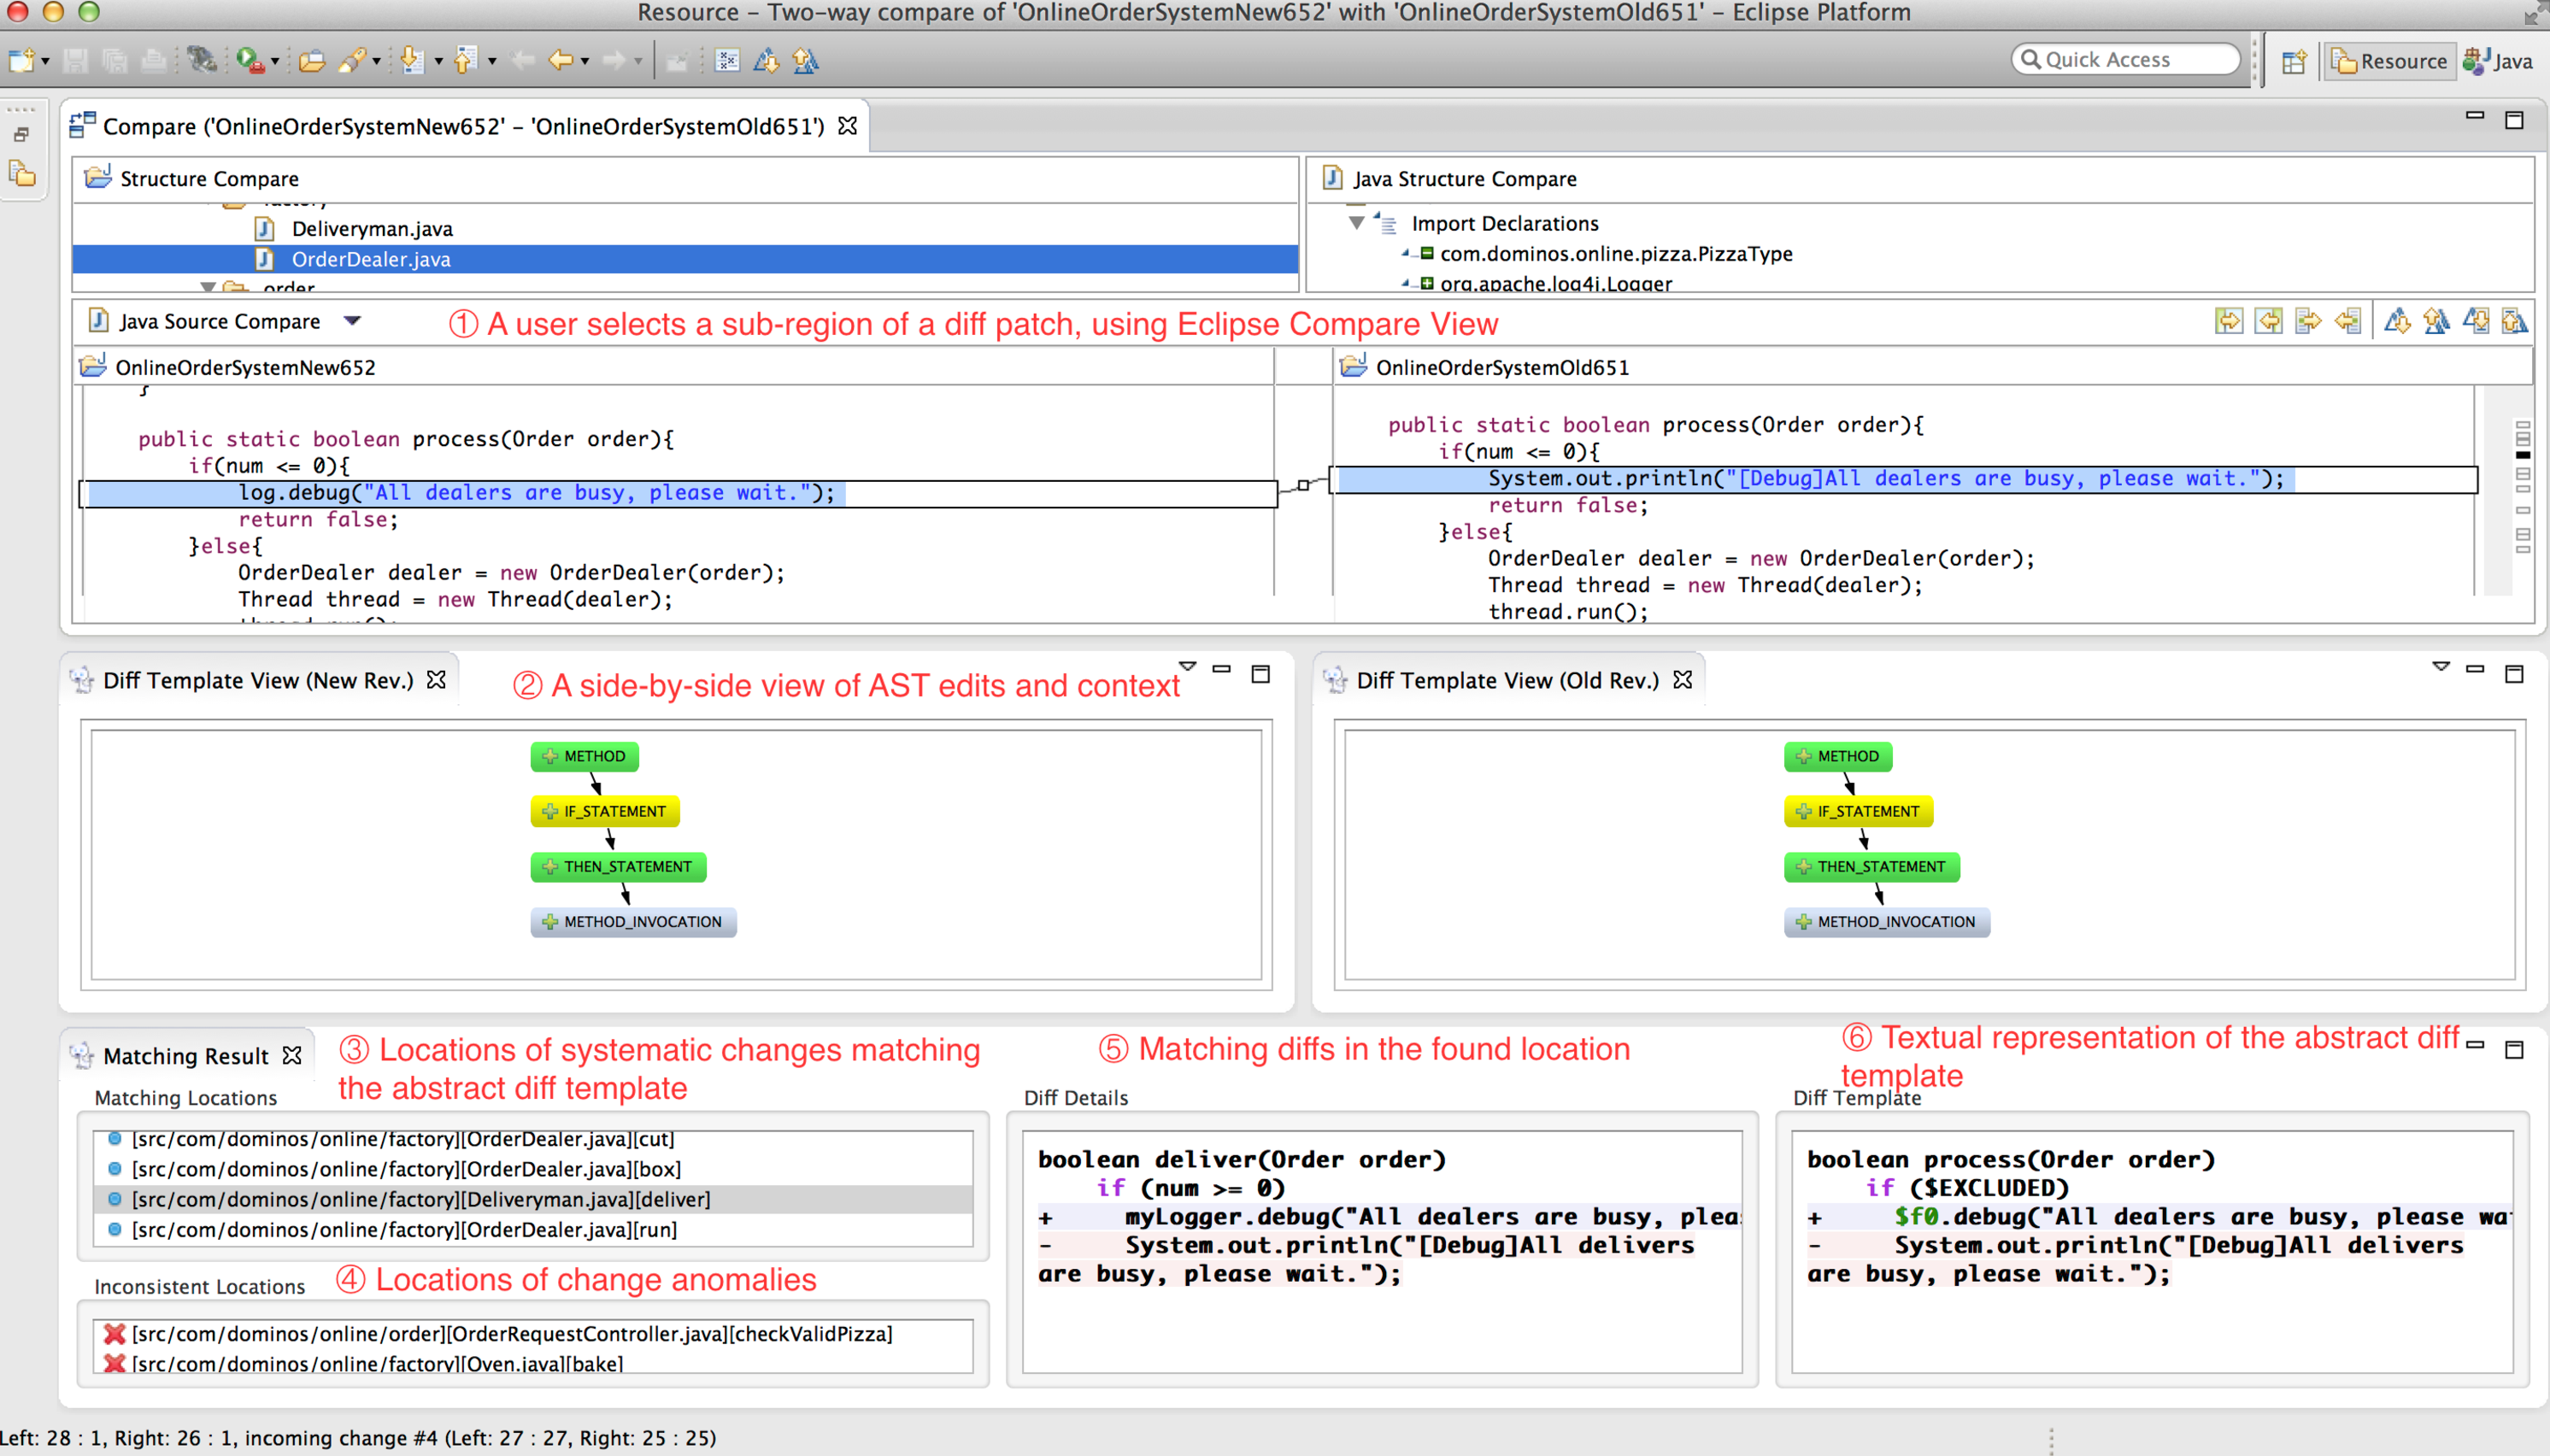
\includegraphics[width=\textwidth]{critics-UI.pdf}
 \caption{A screen snapshot of {\critics}'s Eclipse plugin and its features}
 \label{fig:critics-UI}
\end{figure}

{\critics} is implemented as an Eclipse plugin.\footnote{{\critics}'s tool and evaluation dataset are available online \url{https://sites.google.com/a/utexas.edu/critics/}} Figure~\ref{fig:critics-UI} shows a screenshot of {\critics} plugin. {\critics} is integrated with the {\bf Compare View} in Eclipse, which displays line-level differences per file (see \ding{172} in Figure~\ref{fig:critics-UI}). A user can specify a program change she wants to inspect by selecting the corresponding code region in the Eclipse Compare View. The {\bf Diff Template View} (see \ding{173} in Figure~\ref{fig:critics-UI}) visualizes the change template of the selected change in a side-by-side view. Reviewers can parameterize concrete identifiers and exclude certain program statements by clicking on the corresponding node in the Diff Template View. {\bf Textual Diff Template View} (see \ding{177} in Figure~\ref{fig:critics-UI}) shows the change template in a unified format. The {\bf Matching Result View} summarizes the consistent changes as {\em similar changes} (see \ding{174} in Figure~\ref{fig:critics-UI}) and inconsistent ones as {\em anomalies} (see \ding{175} in Figure~\ref{fig:critics-UI}).

The authors of {\critics} conduct semi-structured interviews with professional developers in industry. All participants strongly affirm that they would like to have Critics integrated into their current code
review environment. Some sample quotes:

\indent {\it``Currently our code review tool only highlights the changed location in a very naive way. A feature like extracting and visualizing the change skeleton can help us better understand the change itself as well as find some underlying change patterns between related changes.''} 

\indent {\it``Since REST APIs across different versions generally share similar code snippets, refactoring on versioned APIs often involve similar changes. Unfortunately these changes are not always exactly the same, including subtle differences in different locations.''}

A controlled lab study shows that human subjects answered code review questions about systematic changes 47.3\% more correctly and 31.9\% faster on average with the assistance of {\critics}, in comparison to the baseline use of the diff and search utilities in Eclipse.

Prior work also observes that developers often submit program changes from multiple programming tasks (e.g., bug fixing, refactorings, feature additions) to a single code review. Reviewers sometimes use ``chunky changes'' or ``code bombs'' to describe such large, unrelated changes that are bundled in a single review. Such changes often lead to difficulty in change comprehension, since reviewers have to mentally ``untangle'' them to figure out which subset of changes addresses which issue first~\cite{kawrykow2011non, murphy2012we, herzig2013impact}. Reviewers have indicated that they can better understand small, cohesive changes rather than large, tangled ones~\cite{rigby2008open}. For example, a code reviewer commented on Gson revision 1154 saying ``I would have preferred to have two different commits: one for adding the new {\ttt getFieldNamingPolicy} method, and another for allowing overriding of primitives.''\footnote{\url{https://code.google.com/p/google-gson/source/detail?r=1154}} This motivates the need of decoupling composite changes in a large code review. 

To address this issue, Barnett et al.~present {\clusterchanges}, a lightweight static analysis technique for decomposing large changes. The insight is that program changes that address the same issue can be related via implicit dependency information such as {\em def-use} relationship. For example, if a method definition is changed in one location and its callsites are changed in two other locations, these three changes are likely to be related and should be reviewed together. Given a code review task, {\clusterchanges} first collects the set of definitions for types, fields, methods, and local variables in the corresponding project under review. Then {\clusterchanges} scans the project for all uses (i.e., references to a definition) of the defined code elements. For instance, any occurrence of a type, field, or method either inside a method or a field initialization is considered to be a use. Based on the extracted def-use information, {\clusterchanges} identifies three relationships between program changes. 

\begin{itemize}
 \item {\bf Def-use relation}. If the definition of a method or a class field is changed, all the uses should also be updated. The change in the definition and the corresponding changes in its references are considered related.
 \item {\bf Use-use relation}. If two or more uses of a method or a class field defined within the change-set are changed, these changes are considered related. 
 \item {\bf Enclosing relation}. Program changes in the same method are considered related because a) based on observation, program changes to the same method are often related, (b) reviewers often inspect methods atomically rather than reviewing different changed regions in the same method separately.
\end{itemize}

Given these relations, {\clusterchanges} creates a partition over the set of program changes by computing a transitive closure of related changes. On the other hand, if a change is not related to any other changes, it will be put into a specific partition, {\em miscellaneous changes}.

Independently from {\clusterchanges}, Tao et al.~present a similar change decomposition technique that leverages more sophisticated heuristics, other than the def-use analysis only~\cite{tao2015partitioning}. Tao et al.~cluster changes based on the following heuristics.

\begin{itemize}
\item {\bf Formatting-only changes.} When formatting is performed together with programming tasks such as bug fixing or feature additions, they isolate formatting changes into a single partition.
\item {\bf Changes with static dependencies.} Tao et al.~use {\em static program slicing}~\cite{weiser1981program} to identify dependencies between program changes. A static slice includes all program statements with {\em data} or {\em control} dependencies. One program statement is data dependent on another statement if the value of its variable is affected by the other. One program statement is control dependent on another statement if the statement may or may not be executed based on the decision of the other statement. If two program changes are applied to the program statements in the same slice, they are considered related to each other.
\item {\bf Changes with similar patterns.} Tao et al.~use pattern matching to identify similar changes that follow the same change pattern, even though there may not exist any static dependency between them. For example, JFreeChart revision 1363 adds three methods {\ttt clearSectionPaints}, {\ttt clearSectionOutlinePaints}, and {\ttt clearSectionOutlineStrokes}. The similarity between these methods' names indicates that they are likely to serve the same purpose. Specifically, two changes are considered similar if 1) they are newly added methods whose names’ similarity is above a threshold $t_m$, or 2) they have the same change type and the similarity between their string contents are above a threshold $t_s$.
\end{itemize}

\bibliography{chapter}
\bibliographystyle{abbrv}
\end{document}
